\documentclass[12pt]{report}
\usepackage{cmap}

\usepackage[T1]{fontenc}
\usepackage[utf8]{inputenc}

\usepackage[english]{babel}
%\usepackage[english,russian]{babel}

\usepackage{hyperref}

\usepackage{amsthm}
\usepackage{amsmath}
\usepackage{amssymb}
\usepackage{amsfonts}
\usepackage{amsthm}
\usepackage{enumerate}
%\usepackage{enumitem}
\usepackage{tikz}
\usepackage{xcolor}
\usepackage{textcomp}

\usepackage{listings}

\usepackage{comment}

\newcommand{\struct}[1]{\textcolor{blue}{#1}}
\newcommand{\Rim}[1]{\uppercase\expandafter{\romannumeral#1}}
\newcommand{\cmd}[1]{\textcolor{blue}{\tt #1}}

\definecolor{mverb}{HTML}{C0E8F8}

\lstnewenvironment{code}[1]{%
  \lstset{backgroundcolor=\color{#1},
  tabsize=10,
  frame=single,
  showlines=true,
  framerule=0pt,
  basicstyle=\ttfamily,
  columns=fullflexible}}{}

\parskip5pt
\parindent0pt

\title% (optional, use only with long paper titles)
{UNIX AND LINIX\\IN INFOCOMMUNICATION\\Week 1}

\author % (optional, use only with lots of authors)
{O.~Sadov%,\\ \texttt{tit@astro.spbu.ru}
}
% - Give the names in the same order as the appear in the paper.
% - Use the \inst{?} command only if the authors have different
%   affiliation.

%%%\institute{ITMO}
%  Университет Информационных Технологий, Механики и Оптики\\
%  кафедра Телекоммуникационных Систем

% - Use the \inst command only if there are several affiliations.
% - Keep it simple, no one is interested in your street address.

\date% (optional, should be abbreviation of conference name)
{Aug 23, 2020 10:33 PM}


\begin{document}
\maketitle
Hi! My name is Oleg Sadov. I'm going to be your instructor for this course.
I've been involved in the Unix world more than 30 years ago and have been
working with Linux systems almost from the very beginning.

This is an Unix and Linux introductory course. This course isn't about
memorizing countless definitions and specifications or endlessly learning
how to keystroke. Instead, we will try to understand the philosophy of systems
and the reasons why existing technical solutions were developed.

This course will provide you with a fundamentals of Unix and Linux operating
systems. It will show you how such systems are organized, and demonstrate
how to use them at an advanced level, which you will be able to practice
on your own. In addition to the usual lectures, we have added additional
materials called ``Under the Hood''. This is not required for graduation checks,
but understanding it does matter when interviewing for a well-known company
like Google or Facebook.

In this course you will be introduced to reasons why open standards and
the open source development model are so important in today's computing
environment. After completing this course, you will have a solid introduction
to working with Unix/Linux from the command line and a good understanding of
principles how these systems work. In applying these skills, you will be able
to perform fundamental operational tasks, whether your Unix/Linux machine is
in your hands or on a remote system across the Internet. And you will be ready
to work with any UNIX-like system with an experienced user and move on
to learning the problems solved by the administrators, developers or DevOps.

\section*{History}

\hbox{\begin{minipage}{0.80\textwidth}
\emph{\struct{{\Large If I have seen further than others,\\
it is by standing upon the shoulders of giants}}}\\
\mbox{}\hfill \emph{\struct{Isaac Newton}}
\end{minipage}\hspace{1em}
\begin{minipage}{0.15\textwidth}
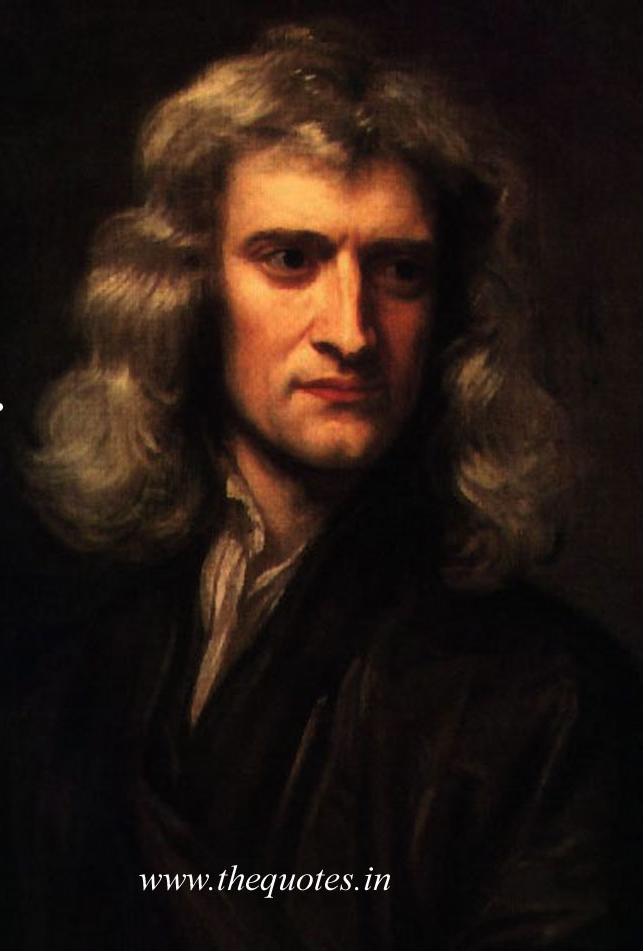
\includegraphics[scale=0.3]{I_Newton.jpg}
\end{minipage}}


Speaking about the history of UNIX and Linux we can recall the well-known
saying~--- \emph{we make our inventions stand on the shoulders of giants}.
But we must understand that many of these giants have failed.
But such fails can be a good lesson for new developers.

\medskip
\hbox{\begin{minipage}[b]{0.2\linewidth}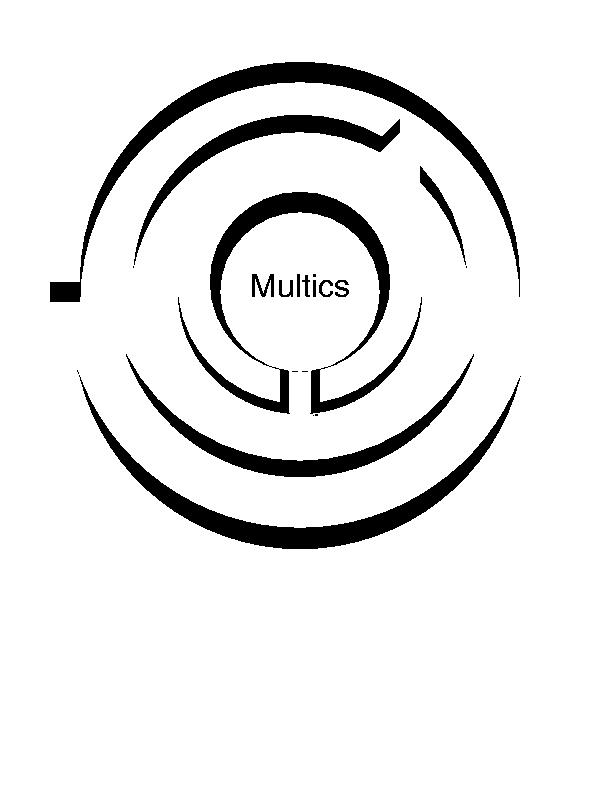
\includegraphics[scale=0.125]{Multics.png}
\end{minipage}
\begin{minipage}[b]{0.8\linewidth}
One such giant was the MULTICS project. The development of Multics began
in 1965 as a research project by MIT, General Electric and Bell Labs to create
a time-sharing, multiprocessing and multiuser interactive operating system.
After several years of development, the enthusiasm of the developers decreased
more and more as the system became more and more complex and the prospects
for completion of development became less and less.
\end{minipage}}

\medskip
\hbox{\begin{minipage}[b]{0.64\linewidth}
Bell Labs pulled out of the project in 1969; but some of the people
who worked on it got a lot of experience. Among them were \struct{Ken Thompson}
and \struct{Dennis Ritchie} of Bell Labs, the inventors of the \struct{UNIX OS}.
\end{minipage}\hspace{1em}
\begin{minipage}[b]{0.32\linewidth}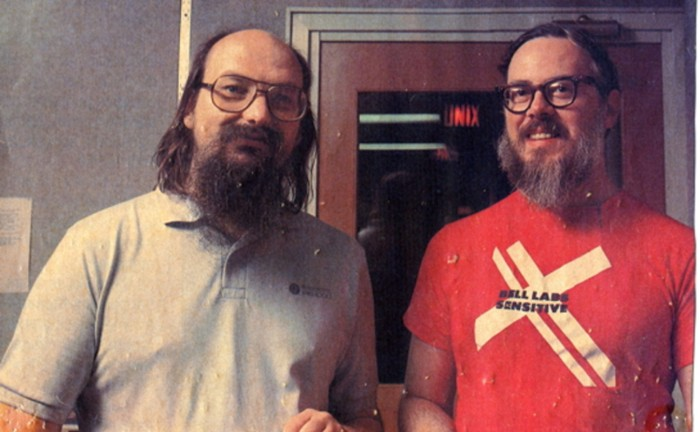
\includegraphics[scale=0.18]{thompson_ritchie.jpeg}
\end{minipage}
}

\medskip
\hbox{\begin{minipage}[b]{0.5\linewidth}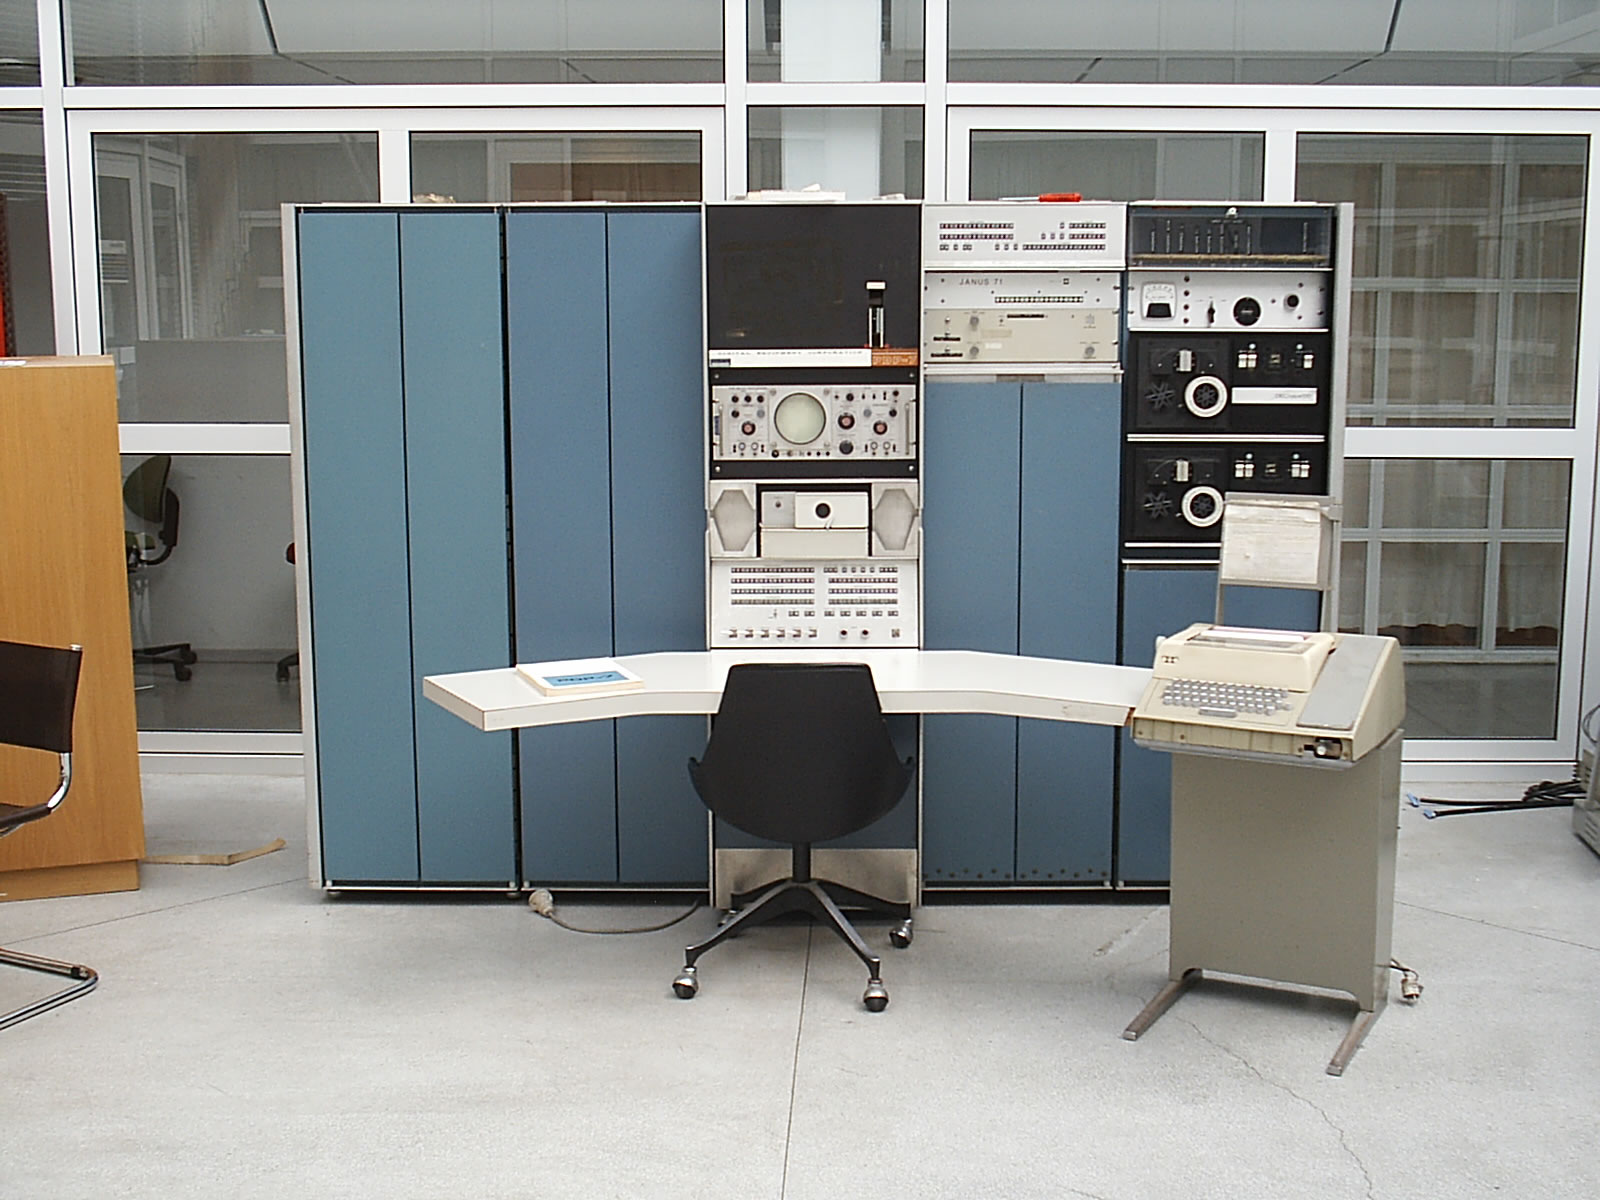
\includegraphics[scale=0.1]{Pdp7-oslo-2005.jpeg}
\end{minipage}\hspace{1em}
\begin{minipage}[b]{0.5\linewidth}
It's funny, but the history of Unix systems is closely related to computer games.
It started in 1969 when Ken Thompson discovered an old \mbox{PDP-7} computer
in a dark corner of the lab and wanted to use it to play Space Travel game.\\\\
\end{minipage}
}

%It's funny, but the history of Unix systems is closely related to computer games.
%It started in 1969 when Ken Thompson discovered an old \mbox{PDP-7} computer
%in a dark corner of the lab and wanted to use it to play Space Travel game.
\medskip
There was little to do~--- an operating system had to be written to run it.
And he did~--- at midnight on \struct{January 1, 1970}, the Unix epoch began.
From this time on, all clocks in UNIX-like systems count down the time,
including your mobile phone. Originally it was a single-tasking OS written
in assembly language that was loaded from paper tapes and called UNICS
as opposed to the complexity of MULTICS.

\href{http://www.levenez.com/unix/}{Unix History Timeline}

\hbox{\begin{minipage}[b]{0.65\linewidth}
And then the team of Ken Thompson and Dennis Ritchie received a new DEC PDP11
computer to develop a word processing system for the Bell Labs patent department.
For the first three months the machine sat in a corner, enumerating all
the closed Knight's tours on a $6\times8$ chess board~---
just because the hard drive wasn't shipped with a super new computer.
This time could be used to choose~a~programming language, because it was
a~computer with a completely new architecture and programs written on PDP7
assembler was not
\end{minipage}\hspace{1em}
\begin{minipage}[t]{0.35\linewidth}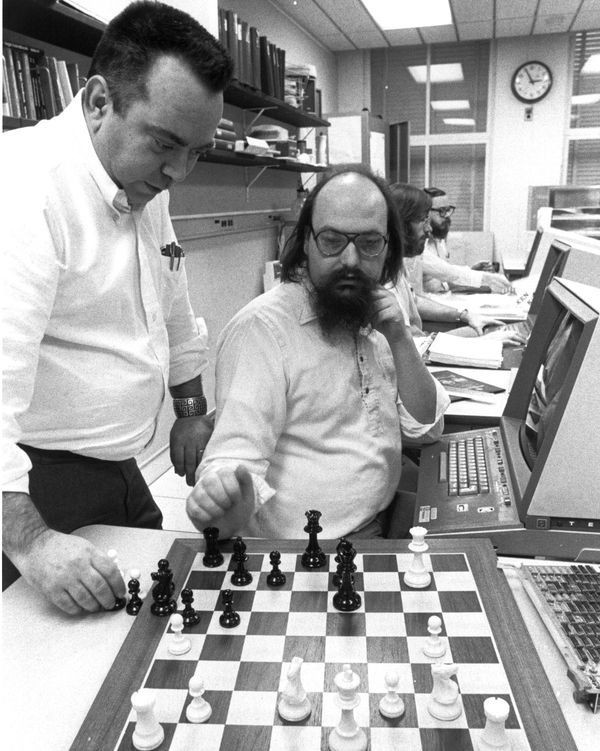
\includegraphics[scale=0.18]{chess.jpeg}
\end{minipage}
}

\noindent
useful for it. And most interesting was the concept of
another project used in some R\&D projects including MULTICS~--- \struct{BCPL}.
It was a high-level programming language focused on portability.
Most of this language was written in the language itself, and only a small
machine-dependent part was written in assembly. To support a new machine,
only 1/5 of the compiler code needed to be rewritten, which usually took
2-5 man-months.

\href{http://www.levenez.com/lang/}{Computer Languages History Timeline}

Thompson used the same concept when writing his simplified successor to BCPL,
language \struct{B}. This language was not very expressive and effective on
the \struct{PDP11}. In 1972, Ritchie started to improve B, which resulted in
creating a new language \struct{C}. In 1973, the UNIX kernel was refactored in C language
to follow the same concept of portability~--- most of the code was machine
independent.
%Finally, they got a very flexible and powerful system with
%a rich set of applications.
\begin{center}
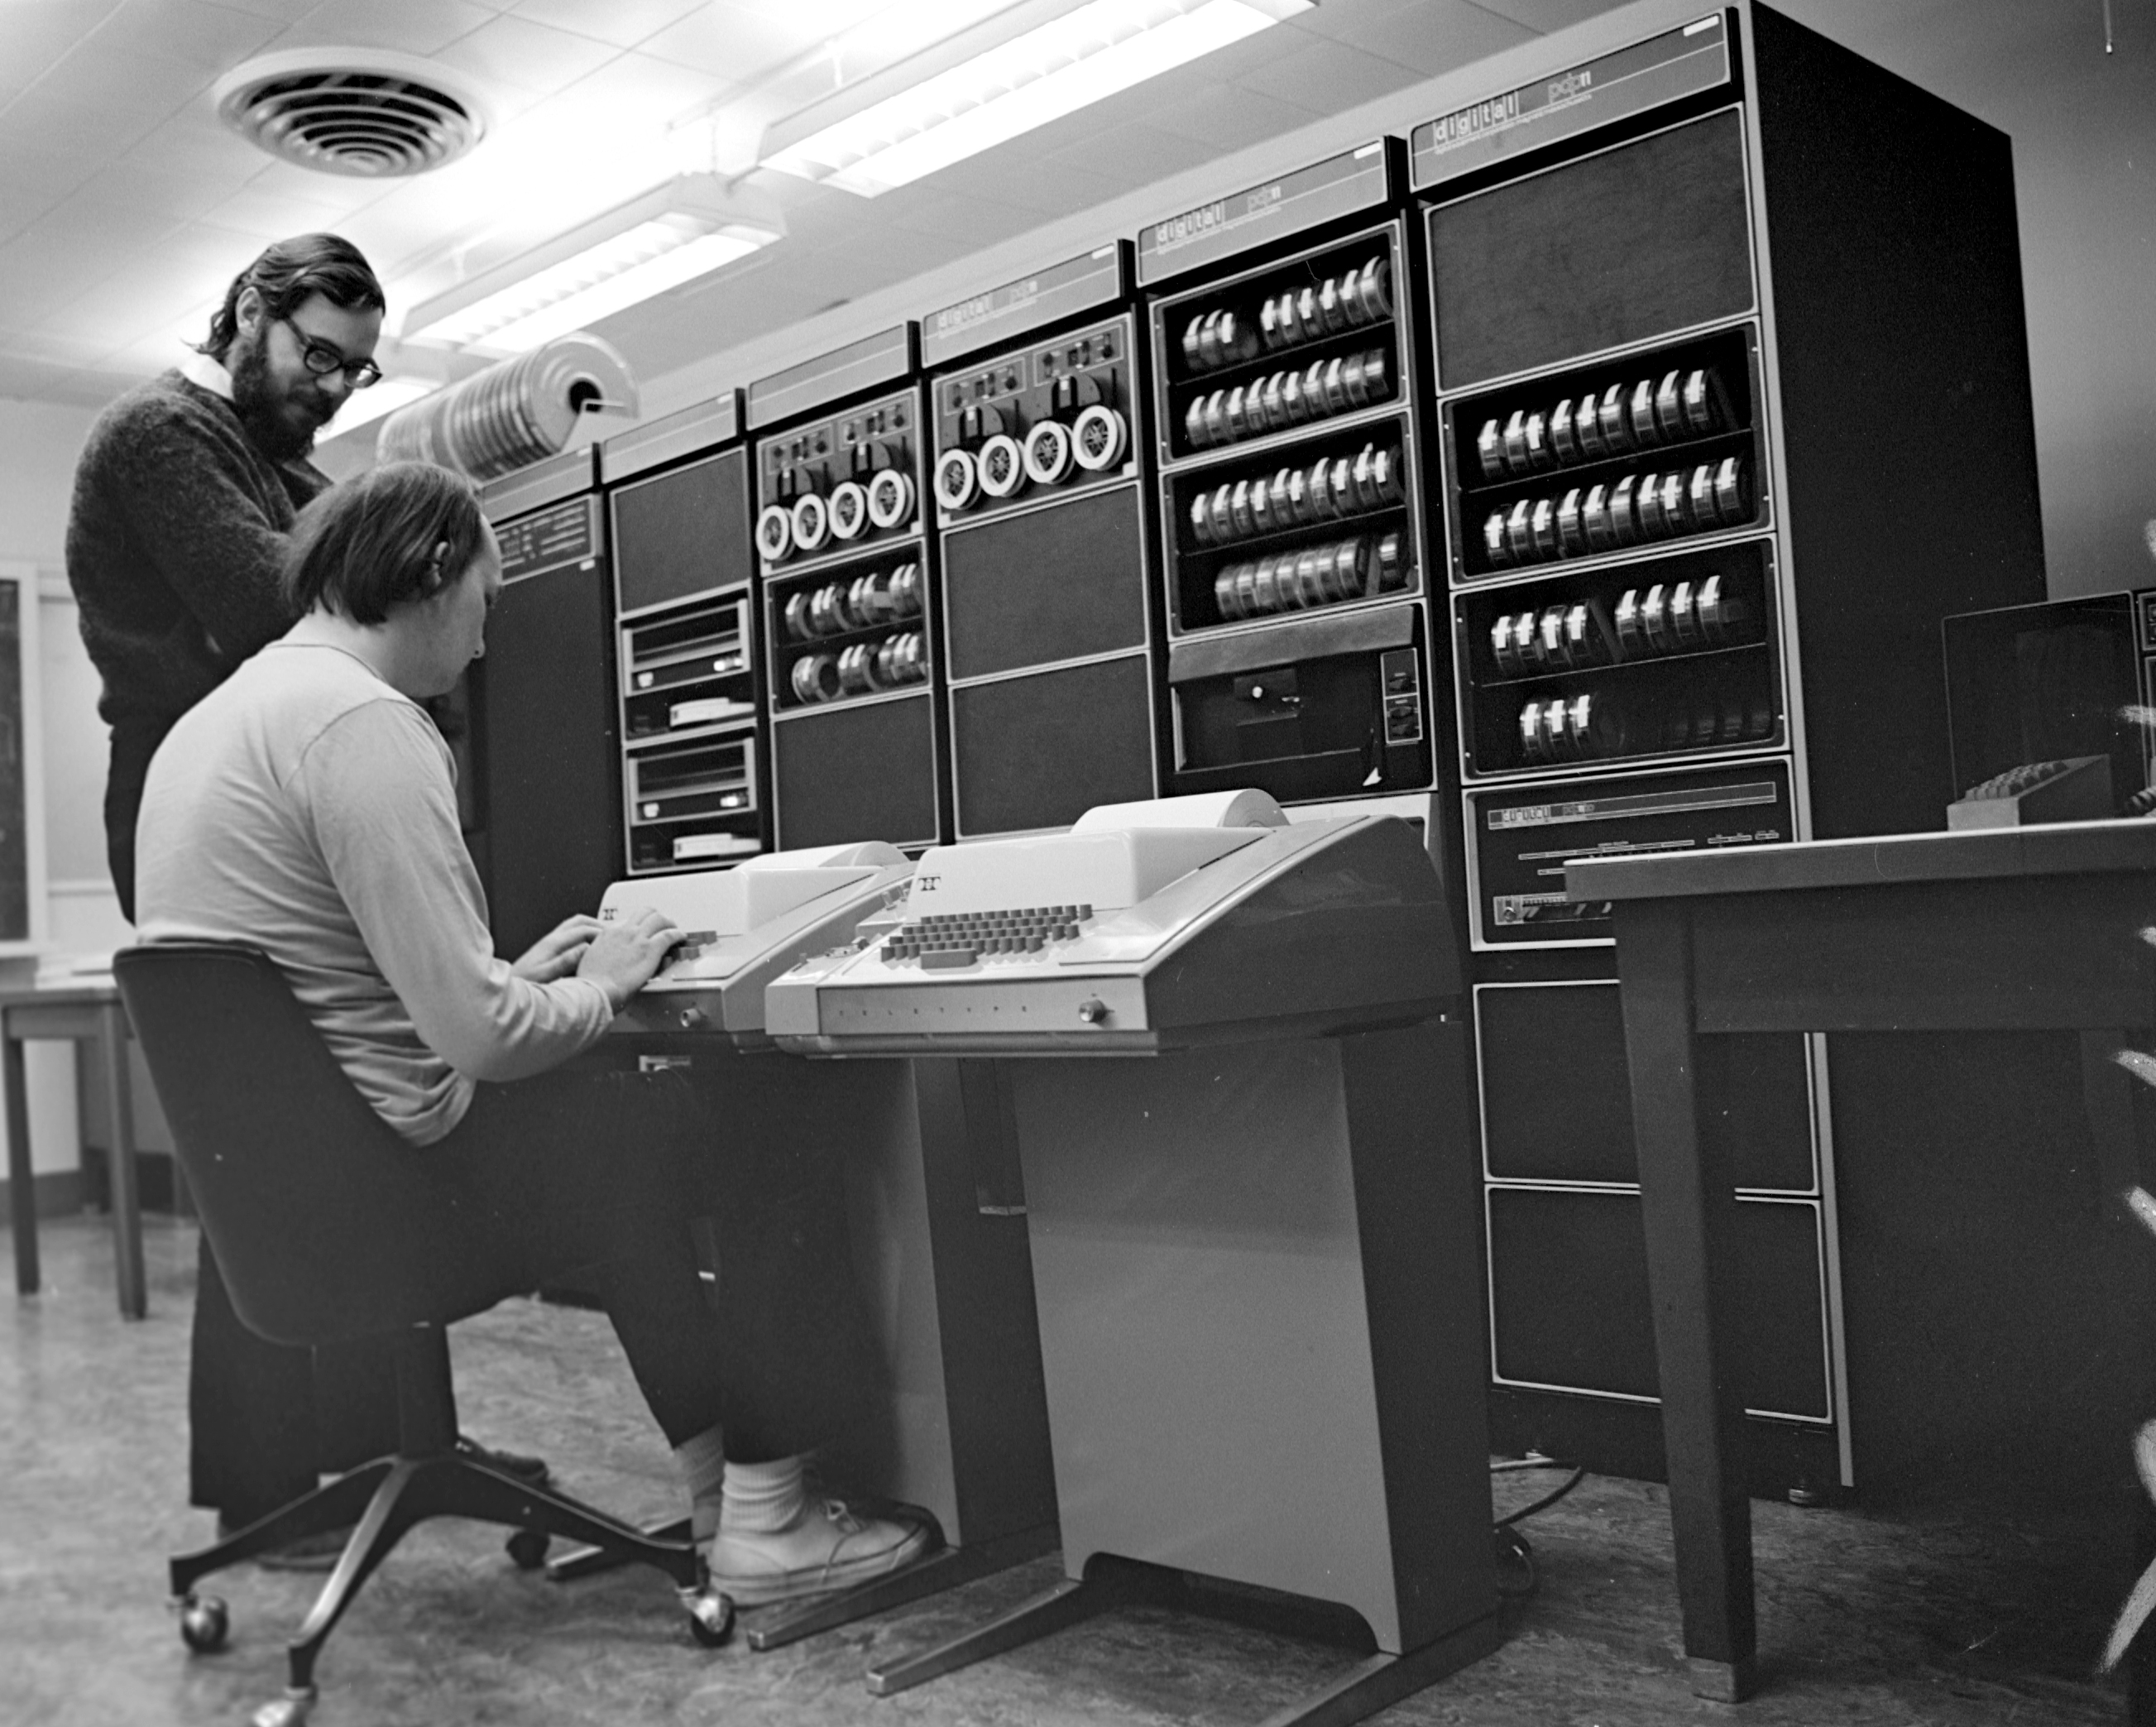
\includegraphics[scale=0.9]{Ken_Thompson__and_Dennis_Ritchie_at_PDP-11.jpg}
\end{center}

The system was distributed in source code among universities for a nominal fee,
which served as an explosive growth in its popularity in the 80s.
Almost all the developers of new computer systems since this period have used
UNIX as the base platform for their new developments. One of the most famous of
these is the Berkeley Software Distribution (\struct{BSD}) developed at
the University of California, Berkeley based on \struct{Unix version 6}
with its \struct{own copyleft license}. And most of the hardware vendors of
the 1980s used BSD as the base OS for their new computers.

UNIX was not a significant part of AT\&T Bell Laboratories' business,
and it was not a problem for them. But in the 1980s Bell Labs split
into several companies as a result of an antitrust lawsuit against AT\&T.
The new UNIX System Laboratories company was created and the new
\struct{UNIX System V} specification was developed. UNIX was the main business
of this company, and they were very aggressive in pushing the new standard in
the market. And that has been the cause of \struct{UNIX wars} against
\struct{non-commercial developers} including BSD.

The commercialization of the UNIX system market and the move to a closed
development and distribution model has led to an alternative movement~---
\struct{GNU}. What is GNU? You know, it's such an African animal. But also it
is a self-referential abbreviation ``\struct{G}NU is \struct{N}ot \struct{U}nix''.
Richard Stallman founded the project in 1978 at MIT. The GNU project is a mass
collaborative initiative for the development of free software. The first
goal of this project was to develop a set of programs similar to
the standard set of utilities in UNIX.

In 1991, a Finnish student \struct{Linus Torvalds} created his own operating
system kernel, which is compatible with the UNIX OS, called \struct{Linux}.
As he said later, ``Just for fun''. The Linux kernel, combined with the set of
utilities from the GNU project, served as the basis for creating a complete
operating system, comparable in capabilities to commercial UNIX systems,
and usually even superior to them.

\medskip
\href{https://www.bell-labs.com/usr/dmr/www/hist.html}%
{\url{https://www.bell-labs.com/usr/dmr/www/hist.html}}

\noindent
\href{https://www.bell-labs.com/usr/dmr/www/chist.html}%
{\url{https://www.bell-labs.com/usr/dmr/www/chist.html}}

\section*{OPEN and FREE SOFTWARE}

Initially, when computer R\&D projects were mostly just university research,
they were open source and free of charge as a common scientific research result.
In addition, scientists were very interested in widespread dissemination of
this result, because their reputation directly depended on the prominence of
their scientific work.

Commercialization has changed this world to a closed and paid model.
Not completely closed, because standardization is very important for
government agencies and corporate consumers to protect investments and
prevent vendor locking. As a consequence, many \struct{open standards} have been
created by committees and organizations: \struct{POSIX}, \struct{ANSI}, \struct{ISO}.

And openness was a serious weapon in business competition. For example,
some well-known companies, including Bull, DEC, IBM, HP, Hitachi, Philips,
Siemens and others, created the Open Software Foundation (OSF) to fight
SUN and AT\&T during the so-called ``Unix wars''. The POSIX subsystem (which
was actually just a description of UNIX-like systems standards) was
included in Microsoft Windows NT because in the 1980s the US federal
government required compatibility with this open standard for government
contracts.

This \struct{openness} is very important because we get more compatible systems
from different vendors, ideally without undocumented features. As a result,
we have a computing infrastructure with higher efficiency and lower cost of
ownership.

But for some people, especially in the scientific world, this is not enough.
And in 1985, \struct{Richard Stallman} from MIT published the GNU Manifesto
where he announced the \struct{GNU Project}. The main goal of this project was
to create a UNIX-like OS with a full set of UNIX utilities from completely
free software. The \struct{Free Software Foundation} (FSF) was formed
to support these activities.

But what is this \struct{freedom} in the computer world and how is it different
with \struct{openness}? This difference is most accurately described in licenses.
In the proprietary world, the most widely used are so-called \struct{copyright
licenses}, which usually restrict certain user rights. Even with legal
access to the source code, the copyright holder can harass the consumer,
as we saw in the USL versus BSD or SCO versus IBM lawsuits.\\
\href{https://www.gnu.org/philosophy/free-software-for-freedom.en.html}%
{\url{https://www.gnu.org/philosophy/free-software-for-freedom.en.html}}

In contrast, the free software world uses copyleft licenses. The most famous
permissive licenses for free software were published in the late 1980s.
Two of them, named BSD and MIT~--- the educational institutions in which
they were created~--- look almost the same and give us the following basic rights:
\begin{itemize}
\item The \struct{freedom to run the program} as you wish, for any purpose
      (freedom 0).
\item The \struct{freedom to study} how the program works, and change it so
      it does your computing as you wish (freedom 1). Access to the source code
      is a precondition for this.
\item The \struct{freedom to redistribute copies} so you can help others
      (freedom 2).
\item The \struct{freedom to distribute copies of your modified versions}
      to others (freedom 3). By doing this you can give the whole community
      a chance to benefit from your changes. Access to the source code is
      a precondition for this.
\end{itemize}

The most famous projects released under these licenses are \struct{BSD Unix} and
the MIT \struct{X-Window} graphics system. Such licenses do not restrict
the use of closed derivative projects and their proprietarization.
To avoid this, the \struct{GNU General Public License} (\struct{GNU GPL} or
\struct{GPL}) was developed. One important limitation added to the fundamental
freedoms of this license (run, learn, share and modify software) is
the limitation for closing. Any derivative work must be distributed under
the same or equivalent license terms.

And the main difference between open-specification software and truly free
software is that we actually have a de facto standard, not a de jure standard.
In free and open source software, we have working reference implementations that
can be used as a basis for future development and cross-testing. % free of charge.

It's interesting, but this license does not completely restrict the creation of
proprietary closed applications using GPL licensed software. For example,
the OS kernel or shared libraries, simply because they are not included
directly in the proprietary application code.

We now have many free and open source licenses approved by
the Open Source Initiative:\\
\href{https://opensource.org/licenses}{\url{https://opensource.org/licenses}}

Another challenge for the free and open world is patent lawsuits.
For example, in 2007, Microsoft threatened to sue Linux companies like Red Hat
over patent violations. To solve this problem \struct{GPLv3} license has been
created, along with some activities such as the Open Invention Network (OIN),
which have a defensive patent pool and community of patent non-aggression
which enables freedom of action in Linux.

\section*{Main Concepts}

At the top level, UNIX-like systems can be very convenient for common
users, and they may not even know they are using this type of OS.
For example, currently the most commonly used operating systems are
Linux-based Android systems and UNIX-based Apple systems, in which
the user only sees the user friendly graphical UI.

But beginners who are just starting to learn UNIX-like systems
for administration or development sometimes complain about their complexity.
Don't be afraid~--- actually such systems are based on fairly simple concepts.
There are only three things (three and a half to be exact) you
need to know to be comfortable with any UNIX-like system:
\begin{itemize}
\item[1)] \struct{Users}
\item[2)] \struct{Files}
\item[3)] \struct{Processes}
\item[3.5)] \struct{Terminal lines}
\end{itemize}

The \struct{users} is not very well known to modern users only because we now
have a lot of computer devices with personal access. UNIX was created at a time
when computers were an expensive rarity and a single computer was used
by many users. As a consequence, from the beginning, \struct{UNIX} had
\struct{strong security policies} and \struct{restrictions on permissions}
for users.

And now on UNIX-like systems, we have dozens of users and groups,
even if hidden by an autologin machinery. And most of them are so-called
\struct{pseudo-users}, which are needed to start system services. As we will see
later, they are required by architecture, since it is on the permissions
of users and groups that the system is built to control access to system
resources (processes and files).

If we are talking about ordinary users, they can log in with a \struct{username}
and \struct{password} and interact with the applications installed on the system.
Each user has full permissions only in their home directory and limited
access rights to files and directories outside of it. This can be viewed
as foolproof~--- common users cannot destroy anything on the system just
because they do not have such permissions. Moreover, they \struct{cannot view}
another user's home directory or protected system files and directories.
To perform system administration tasks, the system has a special
\struct{superuser} (generally called ``\struct{root}'') with extra-permissions.

At the system level, each user or group looks like an integer number:
a~user identifier (\struct{UID}) and a group identifier (\struct{GID}).

\struct{Files} are the next important thing for UNIX-like systems. Almost
all system resources look like files, including devices and even
processes on some systems. And the basic concepts have been the same
since the beginning of the UNIX era. We have a hierarchical file system
with a single root directory. All resources, including file systems
existing on devices or external network resources, are attached to this
file system in separate directories~--- this operation is called
``mount''. On the other hand, you can access a device (real or virtual)
as a stream of bytes and work with it like a regular file. All files and
directories are owned by users (real or pseudo) and groups, and read,
write, and execute access to them is controlled by permissions.

A \struct{process} is a program launched from an executable file. Each process
belongs to a user and a group. The relationship between the owners of
processes and resources determines the access rights according to
the resource permissions. All processes live in a hierarchical system based
on parent-child relationships. There is an initial process on the system
called ``\cmd{init}'' that is started at boot. All system services are started
from this initial process.

There are fundamentally two types of processes in Linux~--- foreground and
background:
\begin{itemize}
\item \struct{Foreground processes} (also referred to as interactive processes)~---
      these are initialized and controlled through a terminal session.
      In other words, there has to be a user connected to the system to start
      such processes; they haven’t started automatically as part of the system
      functions/services.
\item \struct{Background processes} (also referred to as non-interactive/automatic
      processes)~--- are processes not connected to a terminal; they don’t
      expect any user input. System services are always background processes.
\end{itemize}

And finally~--- interactive foreground processes must be attached to
the terminal session through the terminal line. At the time of the creation of
UNIX, a TTY (teletype) device (originally developed in the 19th century),
was the primary communication channel between the user and the computer.
It was a very simple interface that worked with a stream of bytes encoded
according to the ASCII character set. The connection is made via a serial
interface (for example RS232) with a fixed set of connection speeds.

%This interface is still the main user interface for UNIX-like systems.
This interface is still the main user interface for UNIX-like systems.
The implementation of each new form of user interaction, such as
full-screen terminals, graphics systems, and network connections, all
started with the implementation of a simple TTY command line interface.
Moreover, as we will see, this interface abstraction gives us a very
powerful and flexible mechanism for communication between programs,
possibly without human intervention.

\section*{Components}

The main design principle used in UNIX-like systems is the ``\struct{KISS}''
principle. KISS, an acronym for ``keep it stupid simple'' or more officially
``keep it short and simple'', is a design principle noted by the U.S. Navy
in 1960. The KISS principle states that most systems work best if they are kept
simple rather than made complicated; therefore, simplicity should be a key goal
in design, and unnecessary complexity should be avoided.

And from the very beginning UNIX was a very flexible modular system.
The basic set of components from which UNIX-like systems are built is:
\begin{itemize}
\item \struct{Kernel}
\item \struct{Shell}
\item \struct{Utilities}
\item \struct{Libraries}
\end{itemize}

The \struct{kernel} is the first bunch of OS code that is loaded onto your
computer's memory and run for execution. This program launches all
processes on the system, handles interactions between system resources,
and still live while your system is running. The kernel runs with
the highest privileges and has access to all system resources. All processes
in the system operate in user space and interact with such resources and
among themselves, sending requests to the kernel using special software
functions named ``\struct{system calls}''. And the kernel handles such requests
according to the permissions between the processes and resources.

\href{under_the_hood/interrupts.md}%
{Under the hood~--- kernel as a set of interrupt handlers}

But if we have a kernel, it seems reasonable to have a shell around it.
And we have this one. Oh, sorry, not one -- now there are many shells
dating back to the first Unix shell by Ken Thompson, introduced in 1971.
Actually, the \struct{shell} is the first and most important communicator between
human, programs, and kernel. Generally it's just a program that is
launched when the user logs in. It listens for standard input (usually
from the keyboard) and sends the output of commands to standard output
(usually to the screen).

The best-known implementation of the UNIX shell is the \struct{Bourn shell},
developed by Stephen Bourne at Bell Labs in 1979 and included as the
default interpreter for the Unix version 7 release distributed to
colleges and universities. Supported environment variables, redirecting
input/output streams, program pipes and powerful scripting. All modern
shells (and not only UNIX shells) inherit these capabilities from this
implementation.

The shell is a very effective glue for \struct{utilities} in multitasking
operating systems. The most commonly used utilities were developed early
in the life of UNIX. There are tools for working with users, groups, files,
processes. Since UNIX was originally created to automate the work of
the patent department, it has a rich set of tools for processing text files
and streams. The most commonly used design pattern for UNIX utilities is
the filter between standard input and standard output. An arbitrary
number of such programs can be combined into a so-called software
pipeline that uses Shell program pipes for interprocess communication.

Each such utility can be very simple, but together they can be a very
powerful compound program that fits on a single command line. Doug
McIlroy, head of the Bell Labs Computing Sciences Research Center, and
the inventor of Unix pipes, described the Unix philosophy as follows:
``\struct{Write programs that do one thing and do it well. Write programs
to work together. Write programs to handle text streams, because that is
a universal interface.}''

Currently, the most commonly used utilities are those of the GNU project,
which were created after the commercialization of UNIX. In most cases,
they are richer in their capabilities and more complex parameters than
the classic SYSV set of utilities that you see in commercial UNIXes.

On small embedded systems, you might see a systems like ``\struct{busybox}''
that looks like a single binary with many faces built from a configurable
modular library. It may look like a fully featured set of UNIX-style
utilities, including a shell and a text editor. And during the build phase,
you can choose exactly the features you need to reduce the size of
the application.

All utilities and shells are built on top of \struct{software libraries}.
They can be dynamically or statically linked. In the first case,
we have more flexibility for updates and customization and we get a set of
applications that take up less disk/memory space in total. In the second case,
we have a solid state application that is less dependent on the overall system
configuration and can be more platform independent. And as I said earlier
in the first case, you can use libraries with ``viral licenses'' (like the GPL)
to write proprietary applications, but in the second case, you cannot.

\href{under_the_hood/virtual_memory.md}% ***Under the hood -- MMU and shared libraries ***
{Under the Hood~--- Virtual Memory, MMU and shared libraries}

\end{document}

000_intro.tex                  010_input_output_redirect.tex
001_history.tex                011_shell_settings.tex
002_open_free.tex              012_keystrokes.tex
003_main_concepts.tex          013_utilities.tex
004_components.tex  